\lvli{Introduction}

In questo esperimento abbiamo analizzato il comportamento di un FBG (Fiber Bragg Grating). L'FBG sfrutta il Bragg Mirror, ovvero un tipo specifico di photonic crystal che agisce come uno specchio per un determinato range di frequenze. Questo photonic crystall è realizzato come un multilayer film dove vengono alternati due materiali con indice di rifrazione differente. Immaginando un Bragg mirror ideale la lunghezza d'onda riflessa è definita come $\lambda_{BRAGG} = \frac{2\pi}{k_{BRAGG}}$ dove $k_{BRAGG}$ costate di propagazione della fase rispetta questa regola $k_{BRAGG} \cdot (L_1 + L_2) = m \cdot \pi$ con $m \in \mathbb{N}$ e $L_1, L_2$ le due lunghezze dei film. Inserendo un Bragg mirror nella fibra otteniamo un'accoppiamento meccanico trai due in particolare nella compressione e elongazione, infatti tirando la fibra tiriamo anche il mirror e modifichiamo quindi il periodo $(L_1 + L_2)$ che a sua volta modifica $\lambda_{BRAGG}$. Da questo effetto fisico possiamo quindi mettere in relazione l'elungazione con la frequenza riflessa.

Il setup da noi utilizzato è composto da un amplificatore ottico che produce luce a banda larga che viene mandata ad una fibra con l'FBG, la luce riflessa passa poi attraverso un circolatore ottico che la manda ad un analizzatore di spettro (Fig.\ref{fig:setup}).
\begin{figure}[h]
    \centering
    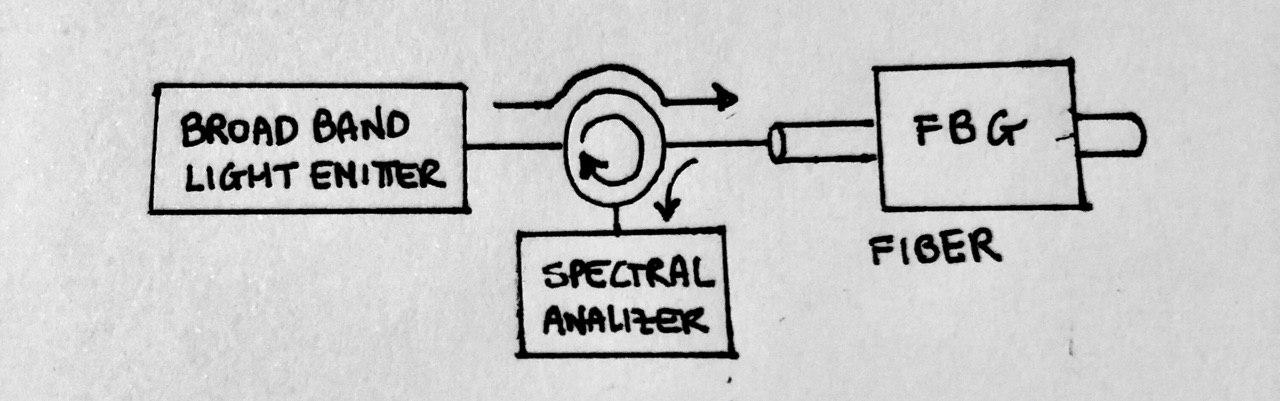
\includegraphics[scale=0.3]{img/setup.jpg}
    \caption{Setup.}
    \label{fig:setup}
\end{figure}

Quello che viene fatto in questo esperimento è misurare la frequenza d'onda riflessa in funzione all'elongazione applicata. In questo caso l'elongazione è realizata girando a mano un tensore circolare (ghiera): ogni rotazione corrisponde ad un'elongazione di $0.5[mm]$ e sulla ghiera ci sono 50 tacche e quindi abbiamo una elongazione di $0.01[mm]$ per tacca. La nostra fibra partiva da una lunghezza di $14[mm]$ ed l'abbiamo elungata di $1.5[mm]$. Le misurazioni da noi eseguite sono riportate in (Tab.\ref{table:measures}), dove per ogni rotazione è stato riportato il valore della frequenza riflessa calcolato a occhio. La tabella presenta tre colonne di misurazione perché sono state fatte più misurazioni consecutive partendo da $14[mm]$ ed arrivando a $14.75[mm]$ poi tornando indietro a $14[mm]$ e poi ritornando a $14.7[mm]$. Nella tabella sono anche specificate con la "x" le misurazioni dove è stato memorizzato lo spettro per l'analisi al calcolatore.
\begin{table}[h]
  \centering
  \begin{tabular}{c|c|c|c}
      Position [mm]  &  $\lambda_B$  [nm]  &  $\lambda_B$  [nm]  &  $\lambda_B$  [nm]  \\
      \hline
      14     &  1534,691     &  1534,682(x)  &  1534,682     \\
      14.05  &  1534.861     &  1534.87      &  1534.861     \\
      14.1   &  1535.032     &  1535.032     &  1535.041(x)  \\
      14.15  &  1535.229     &  1535.186     &  1535.212     \\
      14.2   &  1535.391     &  1535.357     &  1535.391(x)  \\
      14.25  &  1535.604(x)  &  1535.562(x)  &  1535.587     \\
      14.3   &  1535.784     &  1535.749     &  1535.767(x)  \\
      14.35  &  1535.937     &  1535.92      &  1535.946     \\
      14.4   &  1536.125     &  1536.108     &  1536.108(x)  \\
      14.45  &  1536.305     &  1536.262     &  1536.305     \\
      14.5   &  1536.509(x)  &  1536.45 (x)  &  1536.467(x)  \\
      14.55  &  1536.663     &  1536.646     &  1536.646     \\
      14.6   &  1536.851     &  1536.851     &  1536.842(x)  \\
      14.65  &  1537.03      &  1537.005     &  1537.005     \\
      14.7   &  1537.184     &  1537.184     &  1537.184(x)  \\
      14.75  &  1537.389(x)  &  1537.389     &  1537.38      \\

  \end{tabular}
  \caption{Measures.}
  \label{table:measures}
\end{table}
Da una prima analisi otteniamo la curva riportata in (Fig.\ref{fig:firstAnalisy}).
\begin{figure}[h]
    \centering
    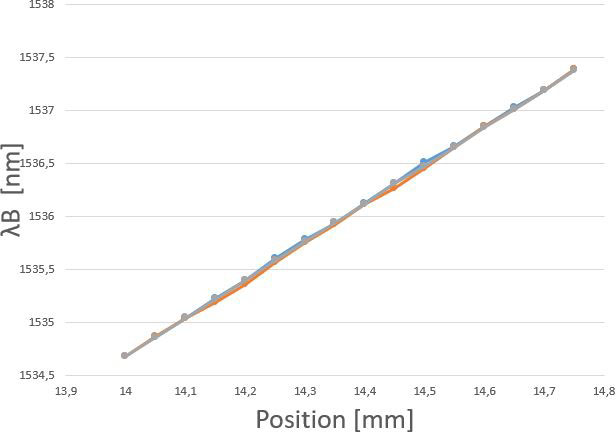
\includegraphics[scale=0.7]{img/firstAnalisy.jpg}
    \caption{First analisy.}
    \label{fig:firstAnalisy}
\end{figure}


\newpage
\lvli{Analysis}
Come prima cosa sono stati importati i 13 file. Essi contengono i dati relativi agli spettri misurati dallo spettrometro e contengono i due valori di frequenza di partenza e step in frequenza in THz, e poi contengono l'elenco di valori potenza riflessa letti. L'importazione è avvenuta convertendo i valori di frequenza in valori di lunghezza d'onda tramite la relazione fisica $\lambda = \frac{c_0}{f}$, ad ognuno di questi valori è stato assegnato il corrispondente valore di potenza in dB come mostrato in (Fig.\ref{fig:spectralPower}). Da questa figura è anche possibile identificare in maniera abbastanza chiara il piccho da analizzare visto che mentre il segnale ha valori inferiori a $-50[dB]$ esso ha un valore di circa $-30[dB]$.
\begin{figure}[h]
    \centering
    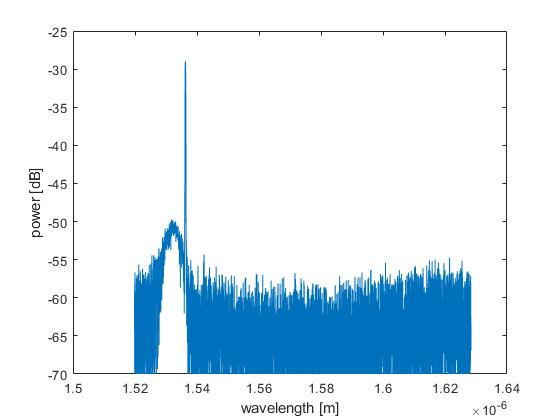
\includegraphics[scale=0.7]{img/spectralPower.jpg}
    \caption{Spectral power for 14[mm] of elongation.}
    \label{fig:spectralPower}
\end{figure}
A questo punto per ogni file viene cercato il valore della lunghezza d'onda corrispondemte al punto di massimo; per migliorare l'analisi viene eseguita un'interpolazione dei punti attraverso una funzione quadratica. Un punto chiave è stato scegliere quali punti considerare nell'approssimazione. Il primo tentativo è stato mediante un'approccio classico, si è scelto di considerare tutti i punti che sono sopra il 90\% del picco che ha comportato una soluzione come in (Fig.\ref{fig:quadratic_fit_scale}), da come si può vedere in questa immagine ci sono un po' di punti intorno al picco che aggiungono del rumore, la scelta successiva sarebbe stata quindi optare per una percentuale maggiore ma così facendo si sarebbe dovuto calcolare a mano per ogni spettro il valore di percentuale ottimale; invece si è scelto un'altro approccio. La soluzione alternativa è stata basata sulla caratteristica di simmetria del picco e segue il seguente approccio: partendo dal punto massimo ci si sposta lateralemente fino a quando non si trovano punti con valori decrescenti, l'esempio di filtraggio dei punti è mostrato in (Fig.\ref{fig:quadratic_fit}).

\begin{figure}[!htb]
  \minipage{0.32\textwidth}
    \centering
    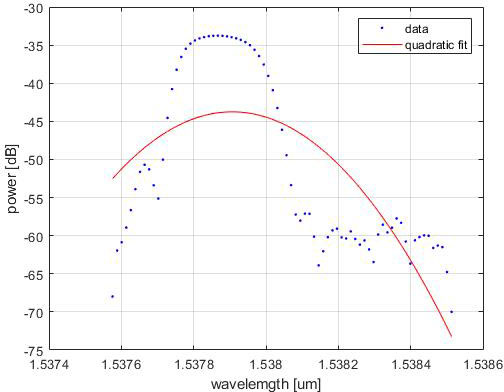
\includegraphics[scale=0.4]{img/quadratic_fit_scale_90.jpg}
    \caption{Quadratic fit scale 90\%.}
    \label{fig:quadratic_fit_scale}
  \endminipage\hfill
  \minipage{0.32\textwidth}
    \centering
    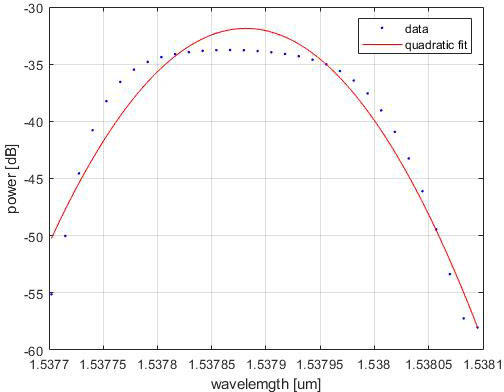
\includegraphics[scale=0.4]{img/quadratic_fit.jpg}
    \caption{Quadratic fit descending cutting mode.}
    \label{fig:quadratic_fit}
  \endminipage
\end{figure}

A questo punto si è messo in relazione i valori delle lunghezze d'onda appena calcolate con in valori di elongazione come mostato in (Fig.\ref{fig:spins}), avendo impostato i $14[mm]$ come nostro valore di 0 otteniamo un'elongazione di $0.75[mm]$. Da qui abbiamo proceduto con un fit lineare per poter ricavare il coefficiente angolare che corrisponde a $a = \frac{\Delta \lambda}{\mu \epsilon} = 3.588 \cdot 10^{-3}$, esso contiene l'informazione della deformazione del FBG che dipende dalla temperatura e dall'elongazione.
\begin{figure}[h]
    \centering
    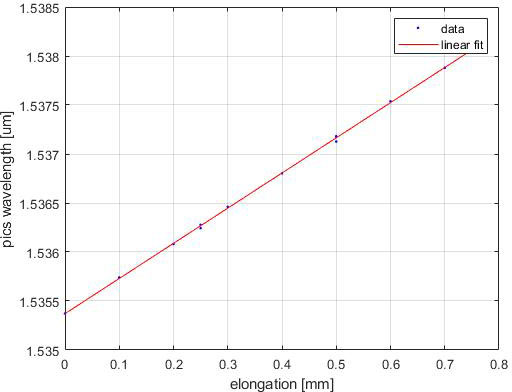
\includegraphics[scale=0.7]{img/spins.jpg}
    \caption{Elongation.}
    \label{fig:spins}
\end{figure}
 Supponendo che la temperatura all'interno della stanza fosse omogenea e che abbiamo svolto l'esperimento in un tempo sufficientemente breve l'effetto della temperatura diventa trascurabile rispetto a quello dell'elongazione. Questo viene anche confermato dall'andamento lineare dei dati ottenuti che si distacca dalla retta di fit di soli $RMSE = 1.6 \cdot 10^{-5}$. Da questo valore possiamo calcolare la sensibility dello strumento mediante la formula:
$$s = \frac{L}{a} = 0.0865[\mu \epsilon]$$
con $L=310.5[mm]$ la lunghezza della fibra a riposo.


\newpage
\lvli{Conclusion}
Il valore ottenuto è molto simile ai valore tipico per sensori di questo tipo:
$$\Delta(\mu\epsilon) = \frac{1 [pm]}{ 1.2 [\frac{pm}{\mu\epsilon}]} \approx 0.8 [\mu \epsilon]$$
L'andamento dei dati raccolti è stato ottimo perché hanno prodotto un andamento lineare come ci aspettavamo con un discostametno di $RMSE = 1.6 \cdot 10^{-5}$. Avendo eseguito le misure sia in contrazione che in elongazione abbiamo avuto la possibilità di controllare l'esistenza o meno di un comportamento di isteresi. I dati raccolti sebbene molto pochi suggeriscono la mancanza di isteresi visto il valore basso di RMSE.

%% DOMANDE PROF
% 1) ho un fattore 10 che non mi torna
% 2) c'è qualche modo in cui possa ricavarmi l'incertezza sulla sensibility?
% 3) c'è altro che si può aggiungere?
% 4) lo spettometro legge potenza? in dB?
